\documentclass[11pt,a4]{article}

\usepackage{url}
\usepackage{graphicx}
\usepackage{natbib}
\usepackage{amsfonts,amsthm}

\def\N{\mathbb{N}}
\newcommand{\sem}{\mathsf{sem}}
\newcommand{\self}{\mathsf{self}}
\newcommand{\produ}{\mathsf{prod}}
\newcommand{\roles}{\mathsf{roles}}
\newcommand{\Neq}{{:}}
\newcommand{\refr}{\mathsf{ref}}
\newcommand{\id}{\mathsf{id}}
\newcommand{\idsem}{\mathsf{idsem}}
\newcommand{\Vars}{\mathsf{Vars}}

\theoremstyle{plain}
\newtheorem{theorem}{Theorem}
\newtheorem{prop}[theorem]{Proposition}
\newtheorem{kor}[theorem]{Corollary}
\newtheorem{lemma}[theorem]{Lemma}
\newtheorem{verm}{Conjecture}

\theoremstyle{definition}
\newtheorem{definition}[theorem]{Definition}
\newtheorem{bem}{Remark}


\title{Sentence generation with RTGs}
\author{Alexander Koller \\ Saarland University \\
  \url{koller@mmci.uni-saarland.de}}
\date{\today\ (v3.0)}

\begin{document}

\maketitle

\section{Introduction}

\section{The generation problem of regular tree grammars}

We start by defining the generation problem of regular tree
grammars. We will first show how RTGs can be equipped with semantic
information; we call the result a \emph{regular generation grammar
  (RGG)} (see Def.~\ref{def:rgg}). Then we will define the
grammatically correct derivations of an RGG, and a \emph{successful}
derivation as one that also achieves a given communicative goal in
Def.~\ref{def:rgg-deriv}. We will then discuss an example in
Section~\ref{sec:rgg-example}.


\subsection{Definitions}

I write $\N_n$ for the set $\{1,\ldots,n\}$.  I write $T_A(B)$ for the
set of terms $f(a_1,\ldots,a_n)$ with $f \in A$ and $a_1,\ldots,a_n
\in B$.  I also assume that the set of nodes in a tree is a set of
strings in $\N^*$ that is closed under left sister (i.e., if $ui$ is a
node of some tree and $i>1$, then $u(i-1)$ is also a node) and prefix
(i.e., if $ui$ is a node of the tree, then $u$ is too).

\begin{definition} \label{def:rgg}
  A \emph{regular generation grammar (RGG)} is a tuple $G =
  (N,\Sigma,S,Pred,R,L)$ consisting of a terminal alphabet $\Sigma$, a
  nonterminal alphabet $N$, a start symbol $S \in N$, a set $Pred$ of
  \emph{predicate symbols}, a set $R$ of \emph{roles}, and a finite
  set $L$ of \emph{lexicon entries} $l = (P,\sem,r)$, where $P = A
  \rightarrow f(B_1,\ldots,B_n)$ is an RTG production rule over $N$
  and $\Sigma$, $r:\N_n \rightarrow R$ an assignment of roles to
  right-hand nonterminal occurrences that assigns the role $\self$ to
  exactly one number, and $\sem \subseteq
  T_{Pred}(\{r(1),\ldots,r(n)\})$ is the semantic representation.
\end{definition}

We write $A \rightarrow f(B_1\Neq r_1,\ldots,B_n \Neq r_n)$ to
abbreviate a production rule with a role assignment that maps $i$ to
$r_i$ for each $1 \leq i \leq n$. We write $\produ(l)$, $\roles(l)$,
and $\sem(l)$ for the production rule, the set of roles
$\{r(1),\ldots,r(n)\}$, and the $\sem$ value of the lexicon entry
respectively.

We will now define the derivations of RGGs. Derivations are sequences
of lexicon entries. It is intuitively clear that the sequence of RTG
production rules in each of these lexicon entries should constitute an
ordinary RTG derivation. Furthermore, we require that there is a
function $\id$ that maps (the position of) a lexicon entry in the
derivation and a role to a variable, and a variable assignment $\refr$
that maps variables to individuals in the universe. For a derivation
to be correct, we insist that the variables assigned by $\id$ are
chosen consistently, i.e.\ if we use some rule $\produ(l_k)$ to expand
a right-hand nonterminal $A \Neq r$ introduced by the rule
$\produ(l_i)$, then the $\self$ variable of $k$ must be the same as
the $r$ variable of $i$.

\begin{definition} \label{def:rgg-deriv}
  Assume a universe $U$ and an infinite set $\Vars$ of variables. A
  \emph{derivation} of a regular generation grammar $G$ is a sequence
  $d = l_1,\ldots,l_n$ of lexicon entries from $G$ such that there are
  functions $\id:\N_n \times R \rightsquigarrow \Vars$ and
  $\refr:\Vars \rightarrow U$ such that
  \begin{enumerate}
  \item grammaticality: the sequence $\produ(l_1),\ldots,\produ(l_n)$
    is a complete RTG derivation that maps $S$ into a tree of terminal
    symbols;
  \item definedness: $\id(i,r)$ is defined iff $r \in
    \roles(l_i)$;
  \item consistent reference: if $\produ(l_k)$ expands the right-hand
    nonterminal $A:r$ in $\produ(l_i)$, then $\id(k,\self) =
    \id(j,r)$;
  \item naming apart: if $r_1,r_2 \in \roles(l_i)$ and $r_1\neq r_2$,
    then $\id(i,r_1) \neq \id(i,r_2)$.
  \end{enumerate}
\end{definition}

We write $\idsem(l_i) = \{P(x_1,\ldots,x_m) \;|\;
\mbox{$P(r_1,\ldots,r_m) \in \sem(l_i)$ and $x_k = \id(i,r_k)$ for all
  $k$}\}$, and take $||S||_M$ to be the set of all variable
assignments $\Vars \rightarrow U$ that satisfy $S$ in all models over
$U$ that satisfy all formulas in the set $M$.

Then we can define a \emph{successful derivation} as a derivation that
also achieves a given communicative goal. We assume two knowledge
bases $SKB$ and $HKB$, which are sets of ground atoms representing the
speaker's and hearer's knowledge, respectively. Then we insist that
the generated statement is truthful (i.e., the semantic
representations of all used lexicon entries are supported by the SKB),
the communicative goal was achieved, and all referring expressions can
be resolved uniquely by the hearer.

\begin{definition} \label{def:rgg-succ-deriv} A \emph{successful
    derivation} of $G$ for the communicative goal $C \subseteq
  T_{Pred}(U)$, the target referent $e \in U$, and the speaker and
  hearer knowledge bases $SKB, HKB \subseteq T_{Pred}(U)$ is a
  derivation $l_1,\ldots,l_n$ of $G$ such that:

  \begin{enumerate}
  \item truthfulness: for all $i$, $\refr(\idsem(l_i)) \subseteq SKB$;
  \item communicative goal achieved: $C \subseteq \cup_{k=1}^n \refr(\idsem(l_k))$;
  \item unique reference: for all $1 \leq i \leq n$ and $r \in
    \roles(l_i)$, $|| \cup_{k=1}^n \idsem(l_k) ||_{HKB}(\id(i,r)) =
    \{\refr(\id(i,r))\}$.
  \end{enumerate}

  The \emph{sentence generation problem} of RGGs is to decide for a
  grammar $G$ and the communicative goal, target referent, and
  knowledge bases, whether there is a successful derivation.
\end{definition}

Compared to a system like SPUD \citep{Stone2003a}, the mapping from
the semantic roles in the lexicon entries to individuals in the
universe is relatively indirect: The semantic roles are first mapped
to variables by the $\id$ function, and then the variables are
assigned individuals by $\refr$. The point about this two-step process
is that it makes it possible to specify the ``unique reference''
condition. By mapping the roles to variables first, we can ask for the
set of all variable assignments that satisfy the combined semantic
representations of all lexicon entries (given the hearer's
knowledge). We can then convince ourselves that the information in the
semantic representations was precise enough that the hearer can
identify the referent uniquely by checking that all these variable
assignments assign the same individual to the variable for the
referring expression, and that this individual is indeed the target
referent. If we had mapped roles to individuals directly, rather than
distinguishing $\refr$ and $\i$, we could have verified that the
assignment satisfies all the semantic representations, but we couldn't
have stated that it is the \emph{only} such assignment.


\subsection{An example} \label{sec:rgg-example}

Let's go through an example to illustrate these definitions.

Consider the following grammar, which is defined over the nonterminals
$\{S, NP, Det, Adj\}$, start symbol $S$, roles $\{\self,
\mathsf{subj}, \mathsf{obj}\}$, and the following lexicon
entries:\footnote{I assume a predicate ``$\cdot = \mathsf{peter}$'' of
  which  $\self = \mathsf{peter}$ is an instance.}

$$\begin{array}{lp{1cm}l}
S \rightarrow \mathrm{likes}(NP \Neq \mathsf{subj}, NP \Neq
\mathsf{obj}) 
&&
Det \rightarrow \mathrm{the} \\
\mathsf{sem} = \{ \mathsf{likes}(\self, \mathsf{subj}, \mathsf{obj})
\} 
&&
\mathsf{sem} = \emptyset \\
&&\\
%
%
NP \rightarrow \mathrm{Peter} 
&&
Adj \rightarrow \mathrm{white} \\
\mathsf{sem} = \{ \self = \mathsf{peter} \}
&&
\mathsf{sem} = \{ \mathsf{white}(\self) \} \\
&&\\
%
%
NP \rightarrow \mathrm{rabbit}(Det \Neq \self, Adj \Neq \mathsf{self})
&&
Adj \rightarrow \epsilon \\
\mathsf{sem} = \{ \mathsf{rabbit}(\self) \}
&&
\mathsf{sem} = \emptyset
\end{array}
$$

\begin{figure}
  \centering
  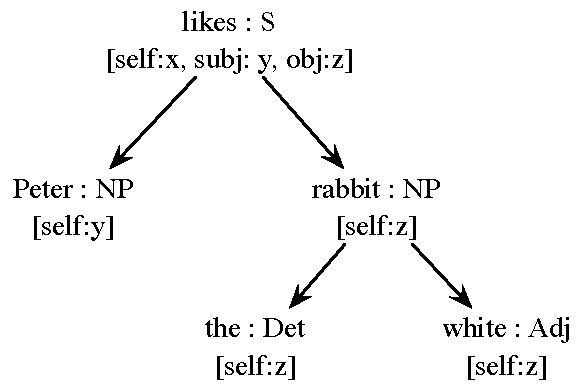
\includegraphics[scale=0.6]{pic-rdg-crisp}
  \caption{Verbalization of the example. Each node displays its
    terminal, nonterminal, and $\id$ function, in this order. $\refr$
    is $\{x \mapsto e, y \mapsto p, z \mapsto r_1\}$.}
  \label{fig:rdg-crisp}
\end{figure}


There are several different derivations for this grammar. Identifying
words with lexicon entries, we can write two of these as:
$$
\begin{array}{lll}
  d_1 &= &(\mathrm{likes}, \mathrm{Peter}, \mathrm{rabbit},
  \mathrm{the}, \mathrm{white}) \\
  d_2 &= &(\mathrm{likes}, \mathrm{Peter}, \mathrm{rabbit},
  \mathrm{the}, \epsilon) 
\end{array}
$$

In each of these cases, we can assume an $\id$ function that looks as
follows:
$$\begin{array}{ll|l}
i&r&\id(i,r) \\\hline
1&\self&x_1 \\
1&\mathsf{subj}&x_2 \\
1&\mathsf{obj}&x_3 \\
2&\self&x_2 \\
3&\self&x_3 \\
4&\self&x_3 \\
5&\self&x_3
\end{array}
$$

The tree represented by the derivation $d_1$ is shown in
Fig.~\ref{fig:rdg-crisp}.  The values of $\refr$ are irrelevant at
this point.

Now let's determine which of these derivations is
\emph{successful}. We assume the following knowledge bases, the
communicative goal $C=\{\mathsf{likes}(e,p,r_1)\}$, and the target
referent $e$.

$$\begin{array}{lll}
  SKB &=
  &\{\mathsf{likes}(e,p,r_1), p = \mathsf{peter}, \mathsf{rabbit}(r_1),
  \mathsf{rabbit}(r_2), \mathsf{white}(r_1)\} \\
  HKB &= &\{p = \mathsf{peter}, \mathsf{rabbit}(r_1),
  \mathsf{rabbit}(r_2), \mathsf{white}(r_1)\} 
\end{array}
$$

Then both $d_1$ and $d_2$ are truthful and convey the communicative
goal for $\refr$ being $\{x_1 \mapsto e, x_2 \mapsto p, x_3 \mapsto
r_1\}$. However, the reference in $d_2$ is not unique: $||\cup
\idsem(l_k)||(x_3)$ is $\{r_1,r_2\}$, i.e.\ the hearer might mistake
the object of the liking as the rabbit $r_2$. Therefore $d_2$ is not
successful. On the other hand, the unique reference condition is
satisfied in $d_1$, and so it is a successful derivation. Thus we can
read off the sentence ``Peter likes the white rabbit'' as a correct
verbalization of $C$ from Fig.~\ref{fig:rdg-crisp}.



\section{RTG generation as planning}


\section{NP-completeness of the RTG generation problem}

\section{Conclusion}




\section*{Version History}

\begin{tabular}{lll}
  v 3.0 & \today & Completely revised \\
  v 2.0 & 29/10/07 & Version for Hector Geffner
\end{tabular}



\bibliographystyle{plainnat}
\bibliography{gen}

\end{document}
